\section{Motivation}
\textbf{
    \begin{itemize}
        \item Discuss the meaning behind silicon hit efficiency.
        \item Why does it need to be measured (high intensity experriment etc)
        \item Why is it done through tracking.
        \item How can this statistic be used?
    \end{itemize}
}
The Mu3e experiment is 

\section{Silicon Hit Inefficiency}
\textbf{
    \begin{itemize}
        \item Reiterate what is meant by silicon hit efficiency.
        \item How is this implemented in the software.
        \item Discuss how this issue might present itself in the experiment.
    \end{itemize}
}
The silicon hit efficiency refers to the proportion of hits that are incident on a sensor and are recorded, for instance a $75\%$ efficient detector would record $75\%$ of the hits that are incident on it. In the software, this inefficiency is introduced when mapping the hits at the track reconstruction level. After the simulation has finished, the hits are collected along with spatial and temporal coordinates. As this mapping process is underway, an inefficient layer is selected, as is a silicon hit efficiency. When the hits in the inefficient layer are being mapped, a random number is used to decide whether the hit is mapped. Under the current algorithm, the inefficiency is introduced as a uniformly distributed frequentist function. 
\begin{equation}
    \text{Hit Efficiency} = \frac{\text{Recorded Hits}}{\text{Number of Hits in Layer}}
\end{equation}
This was chosen for the purpose of understanding the effect that each layer had on the reconstruction.
\section{Ordering of the Algorithm}
\textbf{
    \begin{itemize}
        \item This needs to be cleaned up, with a better title.
        \item Show that the black boxes are what happens in the nominal algorithm.
        \item Reiterate how an inefficieny is simulated and how the backwards propagation works.
    \end{itemize}
}
The ordering of this algorithm is shown below. In order to measure the efficiency of the silicon tracking layers without using truth information and run over real data. As shown in the diagram below, the reconstruction algorithm follows the same process as the nominal reconstruction algorithm. The process uses a series of nested loops to move from each layer and attempt to fit a track to an increasing number of hits. In the diagram, the black boxes represent the common processes between the two algorithms, the red boxes represent the changes that are introduced.
\par
When running over real data, the 'test layer' is skipped and a five-hit track is reconstructed. After the track is reconstructed, the geometric features of the track are used to propagate back to the test layer. Within a specified z and $\phi$ range around the track on the test layer, a hit is either found or not found. It is using this ratio whereby a hit efficiency is calculated.
\usetikzlibrary{arrows,positioning,shapes.geometric}
    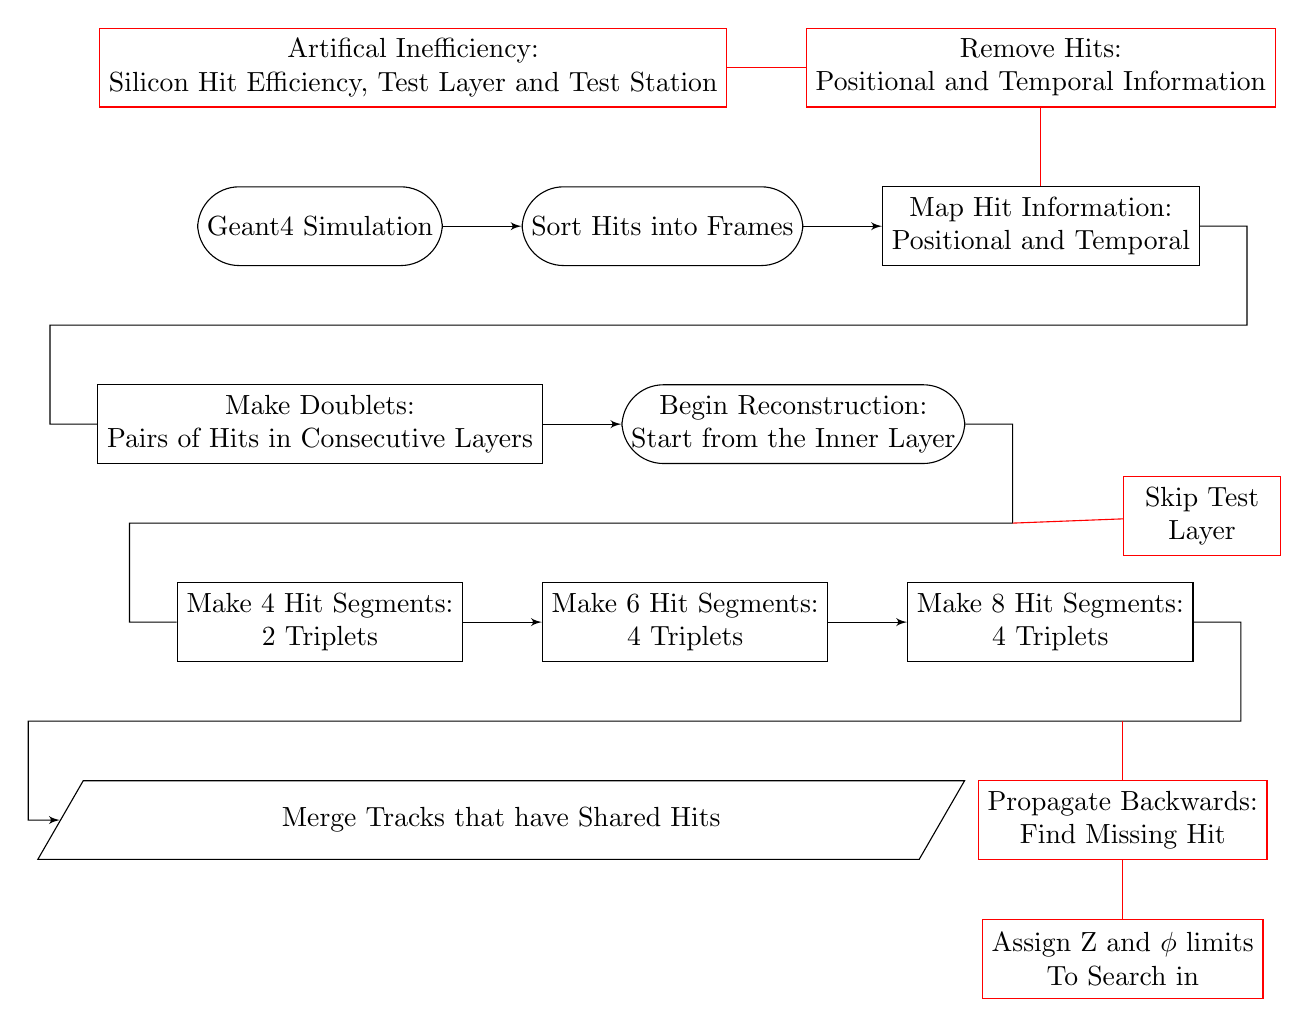
\begin{tikzpicture}[>=latex']
        \tikzset{block/.style= {draw, rectangle, align=center,minimum width=2cm,minimum height=1cm},
        rblock/.style={draw, shape=rectangle,rounded corners=1.5em,align=center,minimum width=2cm,minimum height=1cm},
        input/.style={ % requires library shapes.geometric
        draw,
        trapezium,
        trapezium left angle=60,
        trapezium right angle=120,
        minimum width=2cm,
        align=center,
        minimum height=1cm
    },
        }
        \node [rblock]  (start) {Geant4 Simulation};
        \node [rblock, right =1cm of start] (acquire) {Sort Hits into Frames};
        \node [block, right =1cm of acquire] (rgb2gray) {Map Hit Information: \\ Positional and Temporal};
        \node [block, above =1cm of rgb2gray, draw=red] (mod) {Remove Hits: \\ Positional and Temporal Information};
        \node [block, below =1.5cm of start] (otsu) { Make Doublets: \\ Pairs of Hits in Consecutive Layers};
        \node [rblock, right =1cm of otsu] (gchannel) {Begin Reconstruction:\\Start from the Inner Layer};
        \node [block, below =1.5cm of otsu] (closing) {Make 4 Hit Segments: \\ 2 Triplets};
        \node [block, right =1cm of closing] (hit) {Make 6 Hit Segments: \\ 4 Triplets};
        \node [block, right =1cm of hit] (hits) {Make 8 Hit Segments: \\ 4 Triplets};
        \node [block, left =1cm of mod, draw=red] (mod5) {Artifical Inefficiency: \\Silicon Hit Efficiency, Test Layer and Test Station};
        \node [input, below left=1.5cm and 0.01cm of hit] (limit) {Merge Tracks that have Shared Hits};
        \node [block, below right =0.15 and 2cm of gchannel,draw=red] (mod2) {Skip Test\\ Layer};
        \node [coordinate, below right =0.75cm and 0.6cm of rgb2gray] (right) {};  %% Coordinate on right and middle
        \node [coordinate,above left =0.75cm and 0.6cm of otsu] (left) {};  %% Coordinate on left and middle
        \node [coordinate, below right =0.75cm and 0.6cm of gchannel] (right2) {};  %% Coordinate on right and middle
        \node [coordinate,above left =0.75cm and 0.6cm of closing] (left2) {};  %% Coordinate on left and middle
        \node [coordinate, below right =0.75cm and 0.6cm of hits] (right3) {};  %% Coordinate on right and middle
        \node [coordinate,above left =0.75cm and 5.5cm of limit] (left3) {};  %% Coordinate on left and middle
        \node [coordinate, left =1.5cm of right3] (right4) {};  %% Coordinate on left and middle
        \node [block, below =0.75cm of right4,draw=red] (mod3) {Propagate Backwards: \\Find Missing Hit};
        \node [block, below =0.75cm of mod3,draw=red] (mod4) {Assign Z and $\phi$ limits \\To Search in};

%% paths
        \path[draw,->] (start) edge (acquire)
                    (acquire) edge (rgb2gray)
                    (rgb2gray.east) -| (right) -- (left) |- (otsu)
                    (otsu) edge (gchannel)
                    (gchannel.east) -| (right2) -- (left2) |- (closing)
                    (closing) edge (hit)
                    (hit) edge (hits)
                    (hits.east) -| (right3) -- (left3) |- (limit)
                    
                    ;
        \path[draw=red,-] (mod4) edge (mod3)
                        (mod) edge (rgb2gray)
                        (mod2) edge (right2)
                        (mod3) edge (right4)
                        (mod5) edge (mod)
                    ;
    \end{tikzpicture}

\section{Matching Algorithm}
\textbf{
    \begin{itemize}
        \item Needs to discuss what is defined as a 'matched' track and what a 'truth' track.
        \item Why is it important to measure and have a high matching efficiency? (Picking important parameter range)
        \item What does a high matching efficiency mean for the experiment?
    \end{itemize}
}
When the track is propagated back to the test layer and a hit is either found or not, this ratio of hits found or not found is used to calculate the hit efficiency. In order to trust that this ratio is correct, the track must either match to the nominal algorithm or be a truth track. An algorithm is written such that the tracks are reconstructed together and a matched based on common hits. A track is considered as matched if it either matches to a track reconstructed by the nominal algorithm or it is truth. If it matches to the nominal algorithm, it can be assumed that if a hit is found or not found this can be used to assess the silicon hit efficiency of the layer. If it doesn't match to the nominal tracking but it is a truth track, this can be assumed that it is passing through an intrinsic inefficiency in the layer.
\par
Using this matching algorithm, a matching efficiency can be calculated and plotted against multiple variables associated with the tracks. This is done to find regions in parameter space whereby the matching efficiency is extremely high. By doing this, cuts can be applied when completing the reconstruction over real data and it can be assumed that all the tracks are correct.
\begin{figure}
    \centering
    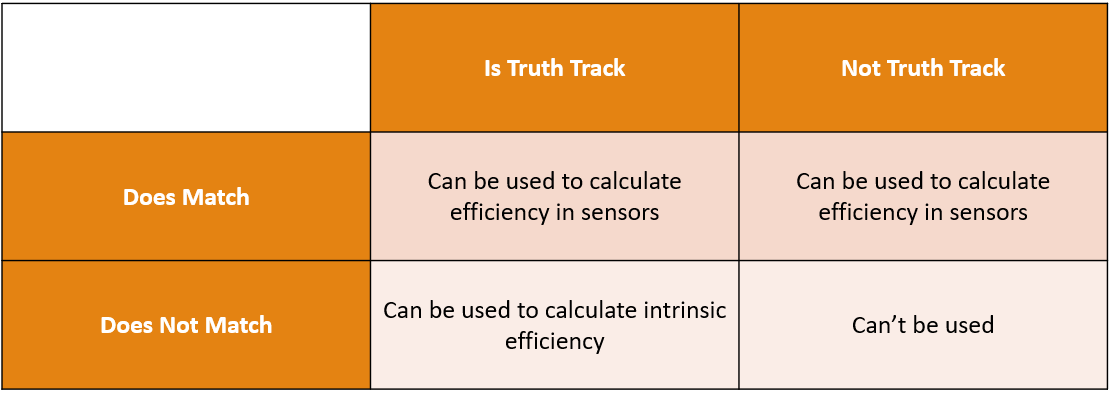
\includegraphics[scale=0.6]{fig/match/Capture.PNG}
    \caption{Table showing the type of track produced by the modified reconstruction algorithm and what it can be used for.}
    \label{fig:table}
\end{figure}
\begin{figure}
    \centering
    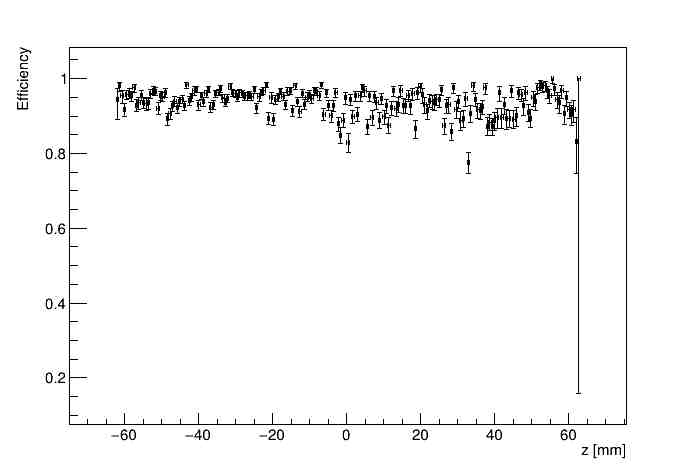
\includegraphics[scale=0.6]{fig/match/prop_z_eff.jpeg}
    \caption{Matching efficiency as a function of prop z.}
    \label{fig:mpz}
\end{figure}
\begin{figure}
    \centering
    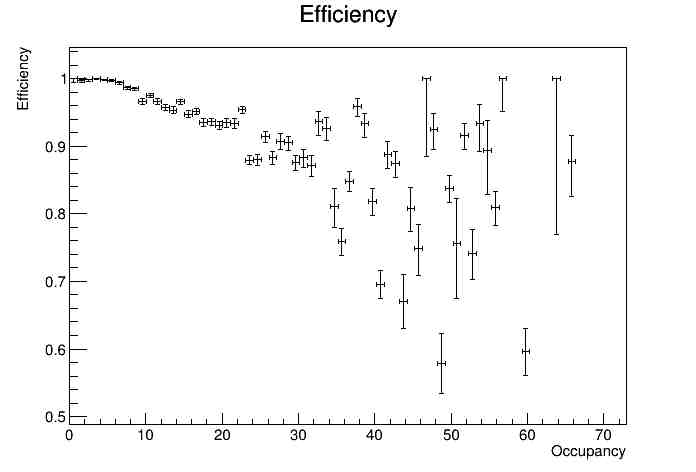
\includegraphics[scale=0.6]{fig/match/effic_nhit.jpeg}
    \caption{Matching efficiency as a function of occupancy.}
    \label{fig:occ}
\end{figure}
\begin{figure}
    \centering
    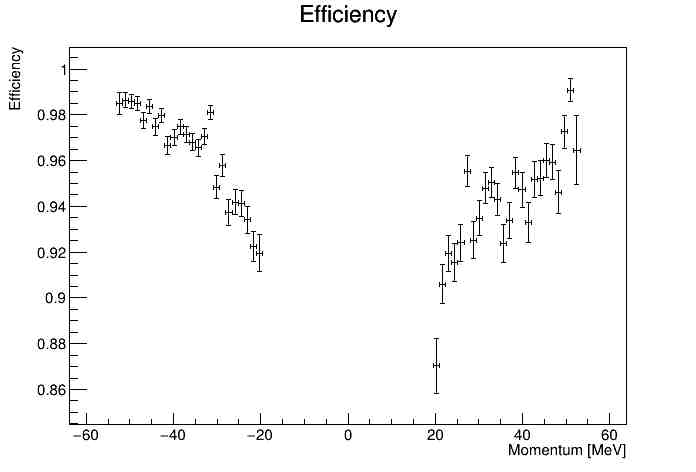
\includegraphics[scale=0.6]{fig/match/effic_p.jpeg}
    \caption{Matching efficiency as a function of momentum.}
    \label{fig:effp}
\end{figure}
\section{Z and $\phi$ Range}
After reconstruction, the parameters of the track are used to propagate the track to a position on the test layer. A preset z and $\phi$ range are then used to locate a hit close to the position of the track. With the assumption that the tracks are either matched to a nominal track or a truth track, if a hit is found or not found, it is because the hit is either there or not there.  Also mention the relationship between the window and the resolution. What is the associated error that will be accumulated if the resolution is improved. 
\begin{figure}
    \centering
    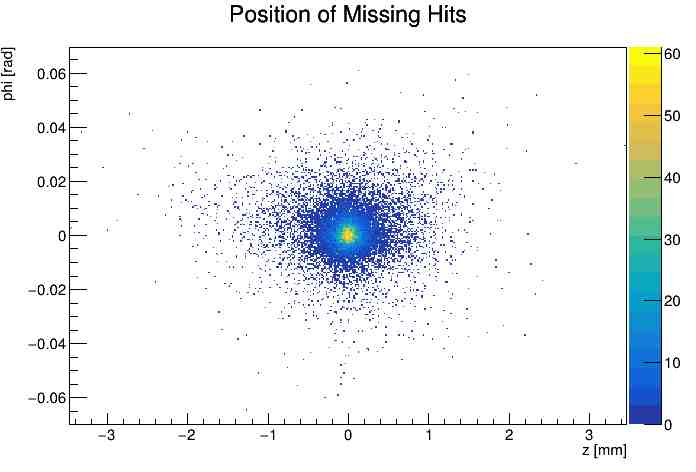
\includegraphics[scale=0.6]{fig/match/position.jpeg}
    \caption{Matching efficiency as a function of momentum.}
    \label{fig:pos}
\end{figure}
\begin{figure}
    \centering
    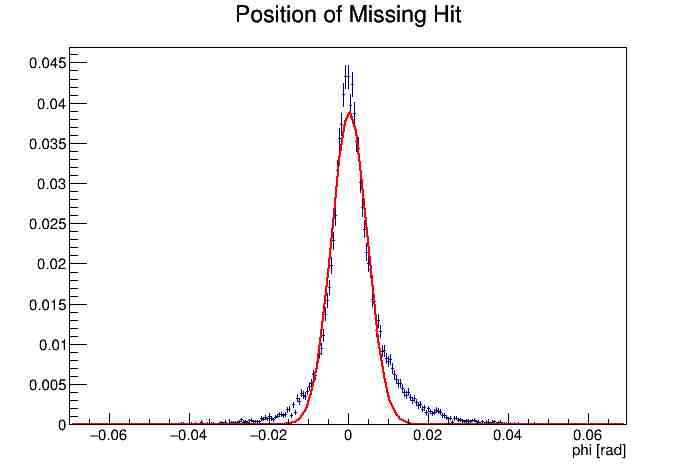
\includegraphics[scale=0.6]{fig/match/position_phi.jpeg}
    \caption{Matching efficiency as a function of momentum.}
    \label{fig:effp}
\end{figure}
\section{Efficiency Heat Maps}
\textbf{
    \begin{itemize}
        \item Go through how the efficiency is calculated.
        \item Move to interesting features (intrinsic inefficiencies and overlap).
        \item Discuss the fiducial region.
    \end{itemize}
}

\begin{figure}
    \centering
    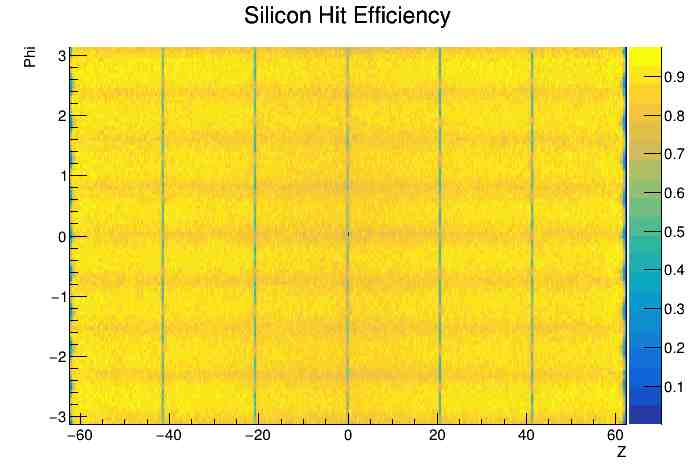
\includegraphics[scale=0.6]{fig/eff/final_eff.jpeg}
    \caption{90\% hit efficiency heat maps.}
    \label{fig:effp}
\end{figure}
\begin{figure}
    \centering
    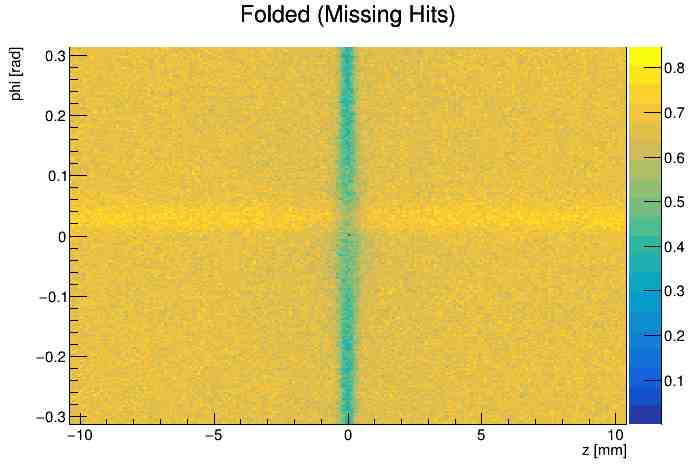
\includegraphics[scale=0.6]{fig/eff/folded_75.jpeg}
    \caption{Folded plot of 75\% hit efficiency.}
    \label{fig:effp}
\end{figure}
\section{Calculation of Hit Efficiency}
\textbf{
    \begin{itemize}
        \item This needs to be completely redone.
        \item The error derivation needs to be done here, Bayesian derivation and error estimation.
    \end{itemize}
}
Go through Bayesian derivation of the errors. Matching efficiency and z and $\phi$ windows
\begin{equation}
    Pr(A|B) = \frac{Pr(B|A)Pr(B)}{Pr(B)}
\end{equation}
\begin{equation}
    Pr(H|M) = \frac{Pr(M|H)Pr(H)}{Pr(M)}
\end{equation}
\section{Effect of Efficiency on Chi Squared Distribution}
\textbf{
    \begin{itemize}
        \item This should be the final stop, the actual presentable effect of an inefficiency.
    \end{itemize}
}
\begin{figure}
    \centering
    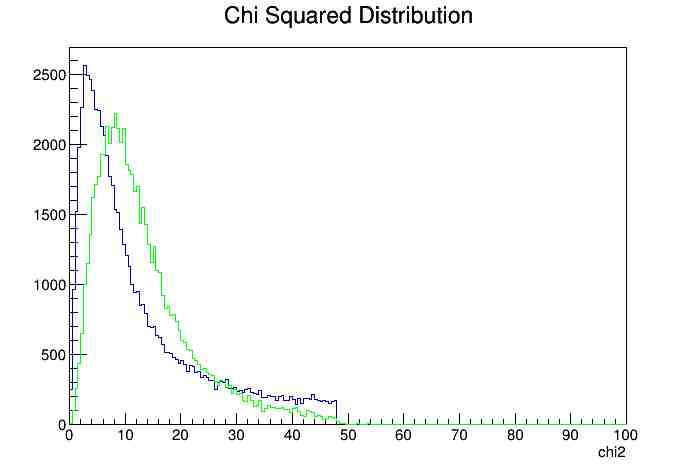
\includegraphics[scale=0.6]{fig/eff/chi2.jpeg}
    \caption{Effect of 70\% efficiency.}
    \label{fig:chi2}
\end{figure}